\chapter{Redox Equilibria and the Nernst Equation}\label{ch:b1:nernst}

Put a zinc strip in a solution of zinc sulfate, a copper strip in a
solution of copper(II) sulfate, join the two solutions by a tube of salt
solution and the two metals by a wire through a light-emitting diode: the
diode lights. The reaction of zinc with copper ions, which in a single
beaker only warms the solution, now drives electrons through a wire. A
battery is this arrangement, packaged; a pH meter and a chloride
electrode are its measuring cousins. This chapter makes the electron
exchange quantitative: \omterm{def:b1:nernst:oxidation-number}{oxidation numbers} to count the electrons,
\omterm{def:b1:nernst:electrode-potential}{electrode potentials} to rank the couples, and the \omterm{thm:b1:nernst:nernst}{Nernst equation} to
follow them with concentration.

\begin{recall}
The school volume (grades 11 and 12) defined \omterm{def:b1:nernst:couple}{oxidants} and \omterm{def:b1:nernst:couple}{reductants},
wrote \omterm{def:b1:nernst:couple}{half-equations}, built cells from two metals and two solutions and
read the zinc--copper cell as a battery. The \omterm{def:b1:extent-q-and-k:quotient}{reaction quotient} and the
equilibrium constant are those of \cref{ch:b1:extent-q-and-k}; activities
are $c/c^\circ$ for solutes and $p/p^\circ$ for gases, 1 for pure solids
and liquids.
\end{recall}

\section{Oxidation numbers and couples}

\begin{definition}[Oxidant, reductant, redox couple, half-equation]\label{def:b1:nernst:couple}
An \emph{oxidant}\index{oxidant} is a species able to gain electrons, a
\emph{reductant}\index{reductant} a species able to give them. An oxidant
Ox and the reductant Red it becomes form a \emph{redox
couple}\index{redox couple} Ox/Red, described by its
\emph{half-equation}\index{half-equation}
$\alpha\,\mathrm{Ox} + n\,\mathrm{e^-} \rightleftharpoons
\beta\,\mathrm{Red}$, balanced in atoms with \ce{H2O} and \ce{H+} when
needed and in charge with the electrons.
\end{definition}

A redox reaction is the exchange of electrons between two couples: the
\omterm{def:b1:nernst:couple}{oxidant} of one is reduced while the \omterm{def:b1:nernst:couple}{reductant} of the other is oxidised,
and the electrons cancel. To count them in a complicated species, each
atom is given an \omterm{def:b1:nernst:oxidation-number}{oxidation number}.

\begin{definition}[Oxidation number]\label{def:b1:nernst:oxidation-number}
The \emph{oxidation number}\index{oxidation number} of an atom in a
species is the charge it would carry if every bond were broken giving
both bonding electrons to the more electronegative atom (shared equally
between two identical atoms). It is written in Roman numerals: iron(III),
\ce{Mn^{+VII}} in the permanganate ion.
\end{definition}

\begin{proposition}[Rules for oxidation numbers]\label{prop:b1:nernst:on-rules}
\begin{enumerate}
  \item An atom in an element has \omterm{def:b1:nernst:oxidation-number}{oxidation number} 0; a monatomic ion has
        its charge.
  \item The \omterm{def:b1:nernst:oxidation-number}{oxidation numbers} of the atoms of a species add up to its
        charge.
  \item Hydrogen is $+$I (except in metal hydrides, $-$I); oxygen is
        $-$II (except in peroxides, $-$I, and bound to fluorine); fluorine
        is $-$I.
  \item In a \omterm{def:b1:nernst:couple}{half-equation} the number of electrons equals the change of
        the \omterm{def:b1:nernst:oxidation-number}{oxidation number} of the element that changes, times the
        number of its atoms.
\end{enumerate}
\end{proposition}

\begin{proof}
1 and 2: breaking all bonds conserves charge, and between identical atoms
nothing is transferred. 3: hydrogen is less electronegative than every
non-metal it bonds to (\cref{ch:b1:periodicity}) and more than the alkali
metals; oxygen is more electronegative than every element but fluorine,
and in \ce{O-O} the shared pair is split. 4: H and O keep their numbers,
so the only atoms whose fictitious charge changes are those of the element
concerned, and the electrons appear in the \omterm{def:b1:nernst:couple}{half-equation} exactly to
balance that change of charge.
\end{proof}

\begin{method}[Oxidation numbers of a species]\label{met:b1:nernst:oxidation-numbers}
Give H, O, F and the ions their usual numbers; the number of the remaining
atom follows from rule 2. In \ce{MnO4-}: $x + 4(-2) = -1$, $x = +7$. In
\ce{Cr2O7^2-}: $2x - 14 = -2$, $x = +6$. In \ce{S4O6^2-}, the average is
$+2.5$; the \omterm{def:b1:lewis-resonance-vsepr:lewis}{Lewis structure} shows two kinds of sulfur.
\end{method}

\begin{method}[Balancing a half-equation]\label{met:b1:nernst:balance-by-on}
\begin{enumerate}
  \item Balance the element that changes \omterm{def:b1:nernst:oxidation-number}{oxidation number}.
  \item Add the electrons: the change of \omterm{def:b1:nernst:oxidation-number}{oxidation number} times the
        number of atoms.
  \item Balance the charge with \ce{H+} (acidic solution) or \ce{OH-}
        (basic solution).
  \item Balance hydrogen and oxygen with \ce{H2O}; check oxygen last.
\end{enumerate}
For the permanganate ion in acid: Mn goes from $+$VII to $+$II, so 5
electrons; the charge on the left is $-1 - 5 = -6$ and on the right $+2$,
so $8\,\ce{H+}$; then $4\,\ce{H2O}$:
\ce{MnO4- + 8H+ + 5e- -> Mn^2+ + 4H2O}.
\end{method}

\section{Electrochemical cells}

\begin{definition}[Electrochemical cell]\label{def:b1:nernst:cell}
An \emph{electrochemical cell}\index{electrochemical cell} is two
\emph{half-cells}\index{half-cell}, each made of a couple and an
electronic conductor, the electrode, joined by an ionic conductor, often a
\emph{salt bridge}\index{salt bridge} (a gel or tube of a concentrated
inert salt such as potassium nitrate). The electrode where oxidation
takes place is the \emph{anode}\index{anode}, the one where reduction
takes place the \emph{cathode}\index{cathode}. The \emph{cell
voltage}\index{cell voltage} is the difference of electric potential
between the two electrodes, positive pole minus negative pole, measured
when no current flows.
\end{definition}

\begin{omfigure}
\begin{tikzpicture}[font=\small, >={Stealth}]
  \pic at (0,0) {beaker={0.7}{omDef!14}};
  \pic at (3.6,0) {beaker={0.7}{omDef!32}};
  \pic at (-0.3,0.25) {electrode={black!35}};
  \pic at (3.9,0.25) {electrode={orange!70!brown}};
  \pic at (0.35,0.55) {saltbridge={2.9}};
  \pic (m) at (1.8,4.3) {meter={V}};
  \draw[thick] (-0.15,2.65) |- (m-a);
  \draw[thick] (4.05,2.65) |- (m-b);
  \node[anchor=east] at (-0.95,1.0) {\ce{Zn}};
  \node[anchor=west] at (4.45,1.0) {\ce{Cu}};
  \node at (0.25,-0.35) {\ce{Zn^2+}, \ce{SO4^2-}};
  \node at (3.6,-0.35) {\ce{Cu^2+}, \ce{SO4^2-}};
  \draw[->, omProp, thick] (-0.15,3.35) -- (0.8,3.35) node[above, midway] {$\mathrm{e^-}$};
  \draw[->, omProp, thick] (2.8,3.35) -- (3.75,3.35) node[above, midway] {$\mathrm{e^-}$};
  \node[anchor=east] at (-0.9,2.3) {$-$ anode};
  \node[anchor=west] at (4.6,2.3) {cathode $+$};
  \node[font=\scriptsize, align=center] at (1.8,2.75) {salt bridge\\ \ce{K+} $\rightarrow$ \quad $\leftarrow$ \ce{NO3-}};
  \node[font=\scriptsize] at (-0.1,-0.8) {\ce{Zn -> Zn^2+ + 2e-}};
  \node[font=\scriptsize] at (3.7,-0.8) {\ce{Cu^2+ + 2e- -> Cu}};
\end{tikzpicture}

{\small The zinc--copper (Daniell) cell. Zinc is oxidised at the \omterm{def:b1:nernst:cell}{anode},
the negative pole; copper ions are reduced at the \omterm{def:b1:nernst:cell}{cathode}, the positive
pole. Electrons flow through the external circuit from zinc to copper;
in the \omterm{def:b1:nernst:cell}{salt bridge} the cations move towards the \omterm{def:b1:nernst:cell}{cathode} and the anions
towards the \omterm{def:b1:nernst:cell}{anode}, keeping each solution neutral.}
\end{omfigure}

A cell is written as a line, \omterm{def:b1:nernst:cell}{anode} on the left: \ce{Zn} $|$ \ce{Zn^2+}
$\|$ \ce{Cu^2+} $|$ \ce{Cu}, single bars for the interfaces, a double bar
for the \omterm{def:b1:nernst:cell}{salt bridge}. With all concentrations at \qty{1}{mol/L} its
voltage is \qty{1.10}{V}. The reaction that runs when the cell delivers
current, \ce{Zn + Cu^2+ -> Zn^2+ + Cu}, is the one that would happen in a
single beaker; separating the \omterm{def:b1:nernst:cell}{half-cells} forces the electrons through
the wire, where they can do work.

\section{Electrode potentials}

A voltage is a difference: only differences between two \omterm{def:b1:nernst:cell}{half-cells} can
be measured. A reference \omterm{def:b1:nernst:cell}{half-cell} is therefore chosen once and for all.

\begin{definition}[Electrode potential, standard potential]\label{def:b1:nernst:electrode-potential}
The \emph{standard hydrogen electrode}\index{standard hydrogen electrode}
is a platinum electrode in contact with hydrogen gas at \qty{1}{bar} and
an ideal solution of \ce{H+} of \omterm{def:b1:extent-q-and-k:activity}{activity} 1. The \emph{electrode
potential}\index{electrode potential} $E$ of a \omterm{def:b1:nernst:cell}{half-cell} is the voltage
of the cell formed with the standard hydrogen electrode on the left:
$E = V_{\text{half-cell}} - V_{\text{SHE}}$. When every species of the
couple has \omterm{def:b1:extent-q-and-k:activity}{activity} 1, it is the \emph{standard potential}\index{standard potential}
$E^\circ$ of the couple, a constant at a given temperature.
\end{definition}

\begin{omfigure}
\begin{tikzpicture}[font=\small, >={Stealth}]
  \pic at (0,0) {beaker={0.72}{omDef!14}};
  % glass jacket, open at the bottom, with the gas inlet on the right
  \draw[om glass] (-0.32,0.35) -- (-0.32,3.0) -- (0.32,3.0) -- (0.32,2.55)
    -- (0.95,2.55) (0.32,2.35) -- (0.95,2.35) (0.32,2.35) -- (0.32,0.35);
  \draw[thick] (0,0.9) -- (0,3.45);
  \fill[black!60] (-0.16,0.5) rectangle (0.16,0.9);
  \foreach \x/\y in {0.45/0.45, 0.55/0.75, 0.48/1.05, -0.45/0.5, -0.52/0.85}
    \draw[omDef!70] (\x,\y) circle (0.055);
  \draw[->] (1.9,2.45) node[right] {\ce{H2}, \qty{1}{bar}} -- (1.0,2.45);
  \draw (0.12,0.7) -- (1.5,0.2) node[right] {platinised platinum};
  \draw (-0.6,1.1) -- (-1.4,1.6) node[left] {\ce{H+}, activity 1};
  \node[anchor=west] at (0.05,3.45) {to the circuit};
\end{tikzpicture}

{\small The \omterm{def:b1:nernst:electrode-potential}{standard hydrogen electrode}: hydrogen gas bubbles over a
platinum plate coated with fine platinum, dipped in a solution where
\ce{H+} has \omterm{def:b1:extent-q-and-k:activity}{activity} 1. Its couple is \ce{H+}/\ce{H2}, of potential 0 by
convention.}
\end{omfigure}

The hydrogen electrode is awkward to use; laboratories measure against a
more convenient \omterm{def:b1:nernst:cell}{half-cell} whose potential is known.

\begin{definition}[Reference electrode]\label{def:b1:nernst:reference-electrode}
A \emph{reference electrode}\index{reference electrode} is a \omterm{def:b1:nernst:cell}{half-cell}
whose potential is fixed and known: the silver--silver chloride electrode
(a silver wire coated with silver chloride in a chloride solution of
fixed concentration) or the calomel electrode (mercury in contact with
\ce{Hg2Cl2} and a chloride solution).
\end{definition}

The table below gives the \omterm{def:b1:nernst:electrode-potential}{standard potentials} used in this volume; the
vertical scale of the next section shows the most common.

\begin{omfigure}
\begin{tabular}{lr@{\qquad}lr}
\hline
couple & $E^\circ$ (V) & couple & $E^\circ$ (V) \\
\hline
\ce{Li+}/\ce{Li} & $-3.04$ & \ce{Cu^2+}/\ce{Cu} & 0.34 \\
\ce{K+}/\ce{K} & $-2.94$ & $[\ce{Fe(CN)6}]^{3-}$/$[\ce{Fe(CN)6}]^{4-}$ & 0.36 \\
\ce{Na+}/\ce{Na} & $-2.71$ & \ce{Cu+}/\ce{Cu} & 0.52 \\
\ce{Mg^2+}/\ce{Mg} & $-2.36$ & \ce{I2}/\ce{I-} & 0.53 \\
\ce{Al^3+}/\ce{Al} & $-1.68$ & \ce{O2}/\ce{H2O2} & 0.69 \\
\ce{Zn^2+}/\ce{Zn} & $-0.76$ & \ce{Fe^3+}/\ce{Fe^2+} & 0.77 \\
\ce{Fe^2+}/\ce{Fe} & $-0.41$ & \ce{Hg2^2+}/\ce{Hg} & 0.80 \\
\ce{Ni^2+}/\ce{Ni} & $-0.24$ & \ce{Ag+}/\ce{Ag} & 0.80 \\
\ce{Pb^2+}/\ce{Pb} & $-0.13$ & \ce{Br2}/\ce{Br-} & 1.08 \\
\ce{H+}/\ce{H2} & 0 & \ce{O2}/\ce{H2O} & 1.23 \\
\ce{S4O6^2-}/\ce{S2O3^2-} & 0.02 & \ce{MnO2}/\ce{Mn^2+} & 1.23 \\
\ce{Cu^2+}/\ce{Cu+} & 0.16 & \ce{Cl2}/\ce{Cl-} & 1.36 \\
\ce{AgCl}/\ce{Ag} & 0.22 & \ce{PbO2}/\ce{Pb^2+} & 1.46 \\
\ce{Hg2Cl2}/\ce{Hg} & 0.27 & \ce{MnO4-}/\ce{Mn^2+} & 1.51 \\
 & & \ce{HClO}/\ce{Cl2} & 1.63 \\
 & & \ce{H2O2}/\ce{H2O} & 1.76 \\
\hline
\end{tabular}

\smallskip
{\small \omterm{def:b1:nernst:electrode-potential}{Standard potentials} at \qty{25}{\celsius}, computed from the
tabulated standard Gibbs energies of formation of the species of each
couple. They may differ by a few hundredths of a volt from other
compilations.}
% ledger: dfg:Li+_ao, dfg:K+_ao, dfg:Na+_ao, dfg:Mg2+_ao, dfg:Al3+_ao, dfg:Zn2+_ao, dfg:Fe2+_ao, dfg:Ni2+_ao, dfg:Pb2+_ao (computed in figdata/bachelor-1/standard-potentials.py)
% ledger: dfg:S4O62-_ao, dfg:S2O32-_ao, dfg:Cu2+_ao, dfg:Cu+_ao, dfg:AgCl_cr, dfg:Cl-_ao, dfg:Hg2Cl2_cr, dfg:Fe_CN63-_ao, dfg:Fe_CN64-_ao, dfg:I-_ao (same script)
% ledger: dfg:H2O2_ao, dfg:Fe3+_ao, dfg:Hg22+_ao, dfg:Ag+_ao, dfg:Br-_ao, dfg:H2O_l, dfg:MnO2_cr, dfg:Mn2+_ao, dfg:PbO2_cr, dfg:MnO4-_ao, dfg:HClO_ao (same script)
\end{omfigure}

\section{The Nernst equation}

\begin{theorem}[Nernst equation]\label{thm:b1:nernst:nernst}
For a couple $\alpha\,\mathrm{Ox} + n\,\mathrm{e^-} \rightleftharpoons
\beta\,\mathrm{Red}$, with possibly other species (\ce{H+}, \ce{H2O},
\ce{Cl-}) on either side, the \omterm{def:b1:nernst:electrode-potential}{electrode potential} is given by the
\emph{Nernst equation}\index{Nernst equation}
\[
  E = E^\circ + \frac{RT}{nF}\ln\frac{\prod a_{\text{ox side}}^{\nu}}{\prod
  a_{\text{red side}}^{\nu}}
  = E^\circ + \frac{0.059}{n}\log\frac{a(\mathrm{Ox})^\alpha\,\cdots}{a(\mathrm{Red})^\beta\,\cdots}
  \quad\text{at \qty{25}{\celsius}},
\]
where each \omterm{def:b1:extent-q-and-k:activity}{activity} carries its \omterm{def:b1:extent-q-and-k:extent}{stoichiometric number} and the factor
$RT\ln 10/F = \qty{0.059}{V}$ at \qty{298}{K}.
\end{theorem}

\admitted{The \omterm{thm:b1:nernst:nernst}{Nernst equation} follows from the relation between the Gibbs
energy of a reaction and the voltage of the cell, derived in the Year~2
volume.}

\begin{example}[Three couples]\label{ex:b1:nernst:examples}
\ce{Cu^2+}/\ce{Cu}: $E = 0.34 + 0.030\log[\ce{Cu^2+}]$ (copper metal has
\omterm{def:b1:extent-q-and-k:activity}{activity} 1).
\ce{Fe^3+}/\ce{Fe^2+}: $E = 0.77 + 0.059\log([\ce{Fe^3+}]/[\ce{Fe^2+}])$.
\ce{MnO4-}/\ce{Mn^2+}: $E = 1.51 + \frac{0.059}{5}\log
\frac{[\ce{MnO4-}][\ce{H+}]^8}{[\ce{Mn^2+}]}$; at equal concentrations of
permanganate and manganese(II), $E = 1.51 - 0.094\,\mathrm{pH}$: the
oxidising power of permanganate falls as the pH rises.
\end{example}

A tenfold change of a concentration moves the potential by $0.059/n$
volt: a few tens of millivolts. This is why a voltage measured to the
millivolt is an accurate measure of a concentration, the principle of the
pH electrode and of the chloride electrode of the weekend problem.

\begin{history}[Walther Nernst]
\begin{minipage}[t]{0.22\linewidth}\vspace{0pt}
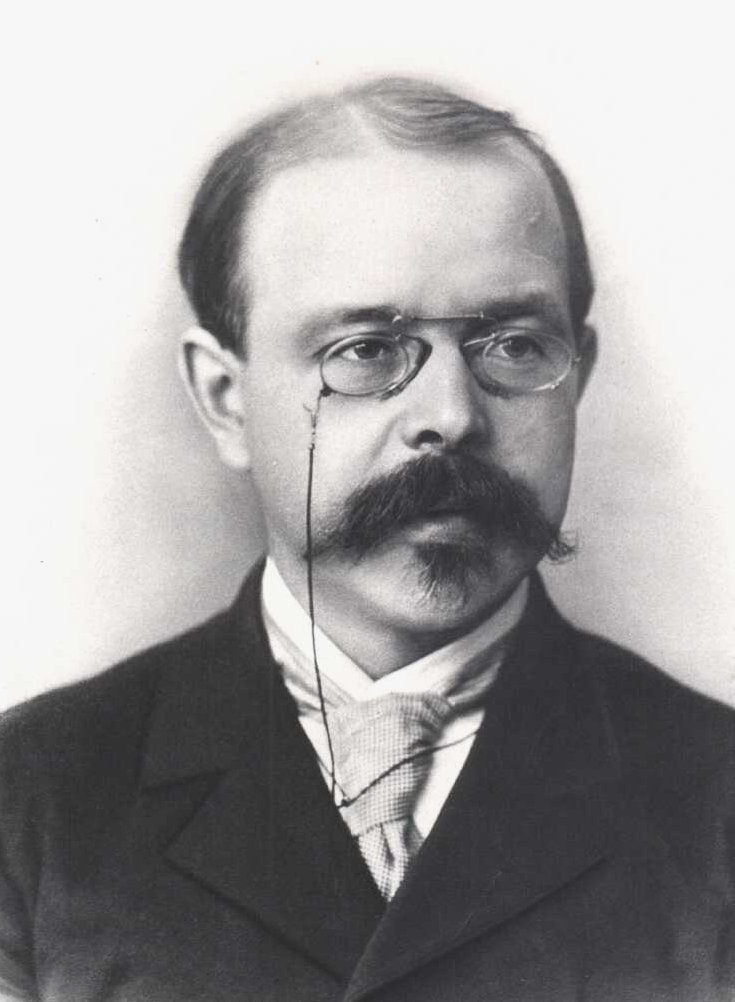
\includegraphics[width=\linewidth]{images/book2/nernst.jpg}
\end{minipage}\hfill
\begin{minipage}[t]{0.74\linewidth}\vspace{0pt}
Walther Nernst (1864--1941), here at twenty-five, in 1889. The equation
of this section, which links the voltage of a cell to the concentrations
of its ions, carries his name, and so does a third principle of
thermodynamics met in the Year~2 volume. (Photograph: Smithsonian
Libraries, public domain, Wikimedia Commons.)
\end{minipage}
\end{history}

\section{Predicting redox reactions}

\begin{method}[Predicting a redox reaction]\label{met:b1:nernst:predict-redox}
\begin{enumerate}
  \item Place the couples on a vertical scale of \omterm{def:b1:nernst:electrode-potential}{standard potentials},
        \omterm{def:b1:nernst:couple}{oxidants} on the left, \omterm{def:b1:nernst:couple}{reductants} on the right.
  \item The strongest \omterm{def:b1:nernst:couple}{oxidant} present (highest $E^\circ$) reacts with the
        strongest \omterm{def:b1:nernst:couple}{reductant} present (lowest $E^\circ$): the arrow from the
        \omterm{def:b1:nernst:couple}{oxidant} down to the \omterm{def:b1:nernst:couple}{reductant}, then up to the products, draws a
        Greek gamma, $\gamma$.
  \item The reaction is favoured ($K > 1$) when the \omterm{def:b1:nernst:couple}{oxidant}'s couple is
        above the \omterm{def:b1:nernst:couple}{reductant}'s; it is \omterm{def:b1:extent-q-and-k:quantitative}{quantitative} in practice when the
        gap exceeds about \qty{0.25}{V} for one exchanged electron.
\end{enumerate}
\end{method}

\begin{omfigure}
\begin{tikzpicture}[font=\small, >={Stealth}, y=2.6cm]
  \draw[->, thick] (0,-1.0) -- (0,1.85) node[above] {$E^\circ$ (V)};
  \foreach \e/\o/\r in {-0.76/\ce{Zn^2+}/\ce{Zn}, 0/\ce{H+}/\ce{H2},
      0.34/\ce{Cu^2+}/\ce{Cu}, 0.77/\ce{Fe^3+}/\ce{Fe^2+},
      1.36/\ce{Cl2}/\ce{Cl-}, 1.51/\ce{MnO4-}/\ce{Mn^2+}} {
    \draw (-0.12,\e) -- (0.12,\e);
    \node[anchor=east] at (-0.25,\e) {\o};
    \node[anchor=west] at (0.25,\e) {\r};
    \node[anchor=west, black!55, font=\scriptsize] at (2.0,\e) {\e};
  }
  \node[omProp] at (-1.0,1.85) {oxidants};
  \node[omDef] at (1.1,1.85) {reductants};
  % the gamma: Cu2+ meets Zn below it on the other side
  \draw[omThm, very thick, ->, rounded corners=4pt] (-1.0,0.28) -- (-1.0,-0.42) -- (0.6,-0.70);
  \draw[omThm, thick, ->] (-0.5,0.40) to[bend left=40] (0.5,0.40);
  \draw[omThm, thick, ->] (0.5,-0.85) to[bend left=40] (-0.5,-0.85);
\end{tikzpicture}

{\small A scale of \omterm{def:b1:nernst:electrode-potential}{standard potentials}. The gamma rule: the \omterm{def:b1:nernst:couple}{oxidant}
\ce{Cu^2+} reacts with the \omterm{def:b1:nernst:couple}{reductant} \ce{Zn} below it on the other side
(thick arrow); \ce{Cu^2+} is reduced to \ce{Cu} (upper curved arrow) and
\ce{Zn} oxidised to \ce{Zn^2+} (lower curved arrow). The reverse reaction,
\ce{Cu} with \ce{Zn^2+}, is not favoured.}
\end{omfigure}

\begin{proposition}[Equilibrium constant from standard potentials]\label{prop:b1:nernst:equilibrium-constant}
For the reaction $\mathrm{Ox_1} + \mathrm{Red_2} \rightleftharpoons
\mathrm{Red_1} + \mathrm{Ox_2}$ exchanging $n$ electrons,
\[
  \log K = \frac{n\,(E^\circ_1 - E^\circ_2)}{0.059}\quad\text{at \qty{25}{\celsius}} .
\]
\end{proposition}

\begin{proof}
At equilibrium no current flows in a cell built from the two couples:
the two electrodes have the same potential, $E_1 = E_2$. Write the \omterm{thm:b1:nernst:nernst}{Nernst
equation} for each with the same $n$: $E^\circ_1 + \frac{0.059}{n}\log
\frac{a(\mathrm{Ox_1})}{a(\mathrm{Red_1})} = E^\circ_2 + \frac{0.059}{n}\log
\frac{a(\mathrm{Ox_2})}{a(\mathrm{Red_2})}$, so $\frac{n(E^\circ_1 -
E^\circ_2)}{0.059} = \log\frac{a(\mathrm{Red_1})a(\mathrm{Ox_2})}{a(\mathrm{Ox_1})
a(\mathrm{Red_2})} = \log K$, the activities being those of equilibrium.
\end{proof}

For the Daniell reaction, $\log K = 2(0.34 + 0.76)/0.059 = 37$: zinc
reduces copper ions completely. For \ce{2Fe^3+ + 2I- <=> 2Fe^2+ + I2},
$\log K = 2(0.77 - 0.53)/0.059 = 8.1$. The criterion of the method
follows: with $n = 1$, a gap of \qty{0.25}{V} gives $K = 10^{4.2}$.

\begin{proposition}[Combining potentials]\label{prop:b1:nernst:combined-potentials}
If the couples $\mathrm{A}/\mathrm{B}$ ($n_1$ electrons) and
$\mathrm{B}/\mathrm{C}$ ($n_2$) combine into $\mathrm{A}/\mathrm{C}$
($n_3 = n_1 + n_2$), then $n_3 E^\circ_3 = n_1 E^\circ_1 + n_2 E^\circ_2$.
Potentials do not add; electron-weighted potentials do.
\end{proposition}

\begin{proof}
In a solution containing A, B and C at equilibrium with one electrode,
the three couples have the same potential $E$. Multiply the \omterm{thm:b1:nernst:nernst}{Nernst
equation} of the first by $n_1$ and of the second by $n_2$ and add: the
\omterm{def:b1:extent-q-and-k:activity}{activity} of B cancels and $(n_1 + n_2)E = n_1E^\circ_1 + n_2E^\circ_2 +
0.059\log\frac{a(\mathrm{A})}{a(\mathrm{C})}$, which is $n_3$ times the
\omterm{thm:b1:nernst:nernst}{Nernst equation} of A/C with $E^\circ_3$ as stated.
\end{proof}

Copper: $2E^\circ(\ce{Cu^2+}/\ce{Cu}) = 0.16 + 0.52 = 0.68$, so
$E^\circ(\ce{Cu^2+}/\ce{Cu}) = 0.34$~V, as in the table. Because
$E^\circ(\ce{Cu+}/\ce{Cu}) > E^\circ(\ce{Cu^2+}/\ce{Cu+})$, the copper(I)
ion oxidises and reduces itself, \ce{2Cu+ -> Cu^2+ + Cu}: it does not
survive in water (\cref{ch:b1:e-ph-diagrams}).

\begin{proposition}[Electrode of the second kind]\label{prop:b1:nernst:second-kind}
A silver wire coated with silver chloride in a chloride solution has the
potential
\[
  E = E^\circ(\ce{AgCl}/\ce{Ag}) - 0.059\log[\ce{Cl-}], \qquad
  E^\circ(\ce{AgCl}/\ce{Ag}) = E^\circ(\ce{Ag+}/\ce{Ag}) - 0.059\,\mathrm{p}K_s(\ce{AgCl}) .
\]
\end{proposition}

\begin{proof}
The wire is in equilibrium with the \ce{Ag+} of the solution:
$E = E^\circ(\ce{Ag+}/\ce{Ag}) + 0.059\log[\ce{Ag+}]$, and silver chloride
fixes $[\ce{Ag+}] = K_s/[\ce{Cl-}]$. Substituting,
$E = E^\circ(\ce{Ag+}/\ce{Ag}) + 0.059\log K_s - 0.059\log[\ce{Cl-}]$.
\end{proof}

Numerically $0.80 - 0.059 \times 9.75 = 0.22$~V, the value of the table
obtained independently from the Gibbs energies. Such an electrode
measures chloride, or, at fixed chloride, serves as a reference.

\section{Exercises}

\begin{exercise}[$\star$]\label{exo:b1:nernst:1}
Give the \omterm{def:b1:nernst:oxidation-number}{oxidation number} of the underlined atom: \ce{\underline{N}H3},
\ce{\underline{N}O3-}, \ce{\underline{S}O4^2-}, \ce{H2\underline{O}2},
\ce{\underline{Cr}2O7^2-}, \ce{\underline{Cl}O-}, \ce{\underline{Fe}3O4}
(average), \ce{\underline{C}H3OH}.
\end{exercise}

\begin{exercise}[$\star$]\label{exo:b1:nernst:2}
Balance in acid the \omterm{def:b1:nernst:couple}{half-equations} of \ce{Cr2O7^2-}/\ce{Cr^3+},
\ce{H2O2}/\ce{H2O}, \ce{O2}/\ce{H2O2} and \ce{SO4^2-}/\ce{SO2}.
\end{exercise}

\begin{exercise}[$\star$]\label{exo:b1:nernst:3}
Write the \omterm{thm:b1:nernst:nernst}{Nernst equation} of \ce{Zn^2+}/\ce{Zn}, \ce{Cl2}/\ce{Cl-},
\ce{O2}/\ce{H2O} and \ce{Hg2Cl2}/\ce{Hg}. Compute the potential of a zinc
strip in \qty{0.010}{mol/L} zinc sulfate.
\end{exercise}

\begin{exercise}[$\star$]\label{exo:b1:nernst:4}
A Daniell cell contains \ce{Zn^2+} at \qty{0.10}{mol/L} and \ce{Cu^2+} at
\qty{0.010}{mol/L}. Compute the potential of each electrode, the \omterm{def:b1:nernst:cell}{cell
voltage}, and say which electrode is the \omterm{def:b1:nernst:cell}{anode}.
\end{exercise}

\begin{exercise}[$\star\star$]\label{exo:b1:nernst:5}
Balance \ce{MnO4- + Fe^2+} in acid, compute its equilibrium constant and
say whether it can serve for a titration.
\end{exercise}

\begin{exercise}[$\star\star$]\label{exo:b1:nernst:6}
Which of these metals dissolve in a \qty{1}{mol/L} acid that is not
itself an \omterm{def:b1:nernst:couple}{oxidant} (hydrochloric acid), giving hydrogen: Mg, Zn, Fe, Ni,
Pb, Cu, Ag? Write the reactions and compute $\log K$ for magnesium and
for iron.
\end{exercise}

\begin{exercise}[$\star\star$]\label{exo:b1:nernst:7}
Iodine titrations use \ce{I2 + 2S2O3^2- -> 2I- + S4O6^2-}. Compute its
constant from the table. Is it \omterm{def:b1:extent-q-and-k:quantitative}{quantitative}?
\end{exercise}

\begin{exercise}[$\star\star$]\label{exo:b1:nernst:8}
From $E^\circ(\ce{Fe^2+}/\ce{Fe}) = -0.41$~V and $E^\circ(\ce{Fe^3+}/\ce{Fe^2+})
= 0.77$~V, compute $E^\circ(\ce{Fe^3+}/\ce{Fe})$. Show that iron(III) ions
react with iron metal and compute the constant.
\end{exercise}

\begin{exercise}[$\star\star$]\label{exo:b1:nernst:9}
Show that the potential of the couple \ce{O2}/\ce{H2O} under \qty{1}{bar}
of oxygen is $1.23 - 0.059\,\mathrm{pH}$, and that of \ce{H+}/\ce{H2}
under \qty{1}{bar} of hydrogen is $-0.059\,\mathrm{pH}$. What is the
voltage of a hydrogen--oxygen fuel cell? Does it depend on the pH?
\end{exercise}

\begin{exercise}[$\star\star\star$]\label{exo:b1:nernst:10}
The copper(I) ion. Using the table, show that \ce{Cu+} disproportionates
in water, compute the constant of \ce{2Cu+ <=> Cu^2+ + Cu}, and the
concentration of \ce{Cu+} left in equilibrium with copper metal and
\ce{Cu^2+} at \qty{0.10}{mol/L}.
\end{exercise}

\begin{exercise}[$\star\star\star$]\label{exo:b1:nernst:11}
A cell \ce{Ag} $|$ \ce{Ag+} (\qty{1.0e-3}{mol/L}) $\|$ \ce{Ag+}
(\qty{0.10}{mol/L}) $|$ \ce{Ag} has the same couple on both sides.
Compute its voltage, identify its poles and describe how the
concentrations evolve while it delivers current. When does it stop?
\end{exercise}

\begin{exercise}[$\star\star\star$]\label{exo:b1:nernst:12}
Hydrogen peroxide. Compute, from the table, the constant of
\ce{2H2O2 -> 2H2O + O2} and explain why a bottle of hydrogen peroxide is
nevertheless stable for months. Which couple of the table makes it an
\omterm{def:b1:nernst:couple}{oxidant}, which a \omterm{def:b1:nernst:couple}{reductant}?
\end{exercise}

\section{Problem: The Electrode that Measures Chloride}

\begin{problem}[{Weekend problem --- oxidation numbers of the silver
chloride couple, a cell against the hydrogen electrode, measuring the
chloride of a water sample, and the standard potential of the
silver--silver chloride electrode}]
\label{pb:b1:nernst:1}
A water laboratory measures chloride with a silver wire coated with silver
chloride, dipped in the sample and connected to a \omterm{def:b1:nernst:reference-electrode}{reference electrode}.
Data at \qty{25}{\celsius}: $E^\circ(\ce{Ag+}/\ce{Ag}) = 0.80$~V,
$E^\circ(\ce{AgCl}/\ce{Ag}) = 0.22$~V, $E^\circ(\ce{Hg2Cl2}/\ce{Hg}) =
0.27$~V, $\mathrm{p}K_s(\ce{AgCl}) = 9.75$, $RT\ln 10/F = 0.059$~V,
$M(\ce{Cl}) = \qty{35.5}{g/mol}$.

\medskip
\noindent\textbf{Part I --- The couple.}
\begin{enumerate}
  \item Give the \omterm{def:b1:nernst:oxidation-number}{oxidation number} of silver in Ag, \ce{Ag+} and \ce{AgCl},
        and that of chlorine in \ce{AgCl} and \ce{Cl-}.
  \item Write the \omterm{def:b1:nernst:couple}{half-equation} of the couple \ce{AgCl}/\ce{Ag}.
  \item Write its \omterm{thm:b1:nernst:nernst}{Nernst equation}.
  \item Explain why the potential depends only on the chloride
        concentration.
  \item What is the potential of the electrode in \qty{1.0}{mol/L}
        chloride?
  \item Compute it in \qty{0.010}{mol/L} chloride.
\end{enumerate}

\medskip
\noindent\textbf{Part II --- A cell against the hydrogen electrode.}
\begin{enumerate}[resume]
  \item Write the cell formed by the \omterm{def:b1:nernst:electrode-potential}{standard hydrogen electrode} and the
        silver chloride electrode in \qty{0.10}{mol/L} chloride.
  \item Which electrode is the positive pole?
  \item Compute the \omterm{def:b1:nernst:cell}{cell voltage}.
  \item Write the reaction that runs when the cell delivers current.
  \item Compute its equilibrium constant.
  \item In which direction do the electrons move in the wire?
\end{enumerate}

\medskip
\noindent\textbf{Part III --- Measuring chloride.}
The reference is a calomel electrode in \qty{1.0}{mol/L} potassium
chloride.
\begin{enumerate}[resume]
  \item What is the potential of the reference?
  \item For a sample at \qty{1.0e-3}{mol/L} chloride, which electrode is
        the positive pole, and what is the voltage?
  \item Express the voltage $U$ (silver electrode minus reference) as a
        function of $[\ce{Cl-}]$.
  \item A sample gives $U = \qty{0.115}{V}$. Compute its chloride
        concentration in \unit{mol/L} and \unit{mg/L}.
  \item An error of \qty{1}{mV} on $U$ gives what relative error on the
        concentration?
  \item Below what chloride concentration does the electrode stop
        following the \omterm{thm:b1:nernst:nernst}{Nernst equation}, its silver chloride dissolving?
\end{enumerate}

\medskip
\noindent\textbf{Part IV --- Where does 0.22 V come from?}
\begin{enumerate}[resume]
  \item Write the \omterm{thm:b1:nernst:nernst}{Nernst equation} of \ce{Ag+}/\ce{Ag}.
  \item In the presence of solid silver chloride, express $[\ce{Ag+}]$ as a
        function of $[\ce{Cl-}]$.
  \item Deduce the potential of the silver wire as a function of
        $[\ce{Cl-}]$.
  \item Identify $E^\circ(\ce{AgCl}/\ce{Ag})$ in this expression.
  \item Compute it from $E^\circ(\ce{Ag+}/\ce{Ag})$ and $\mathrm{p}K_s$, and
        compare with the value of the table.
  \item State the \omterm{def:b1:nernst:electrode-potential}{standard potential} of the silver--silver chloride
        electrode to two decimals.
\end{enumerate}
\end{problem}
